% !TEX root = ./report.tex

\clearpage
\section{Background}
\label{background}

\subsection{The Regionalized Value-State Dependence Graph}
\label{background:RVSDG}

The \textit{Regionalized Value-State Dependence Graph} (RVSDG) is a
\textit{directed acyclic graph} (DAG) \textit{demand-based dependence graph}
(DDG), consisting of nodes representing computations and edges representing the
dependencies between nodes. Each node has inputs and outputs connected through
edges. The arity and order of inputs and outputs depend on the operation the
node represents.

The RVSDG has two kinds of nodes, and two kinds of edges: simple- and complex-
nodes, and data- and state- dependency edges. Simple nodes represent ``basic
operations'', such as addition and subtraction. Complex nodes contain another
RVSDG subgraph, and are also called \textit{regions}.

\subsubsection{Edges}

The RVSDG has two types of edges: data dependence edges, and state dependence
edges, representing data and state dependencies respectively. Data dependence
edges represent a data dependency one node has to another. State dependence
edges are used to preserve the program semantics when it has side-effecting
operations. We use dashed lines in this report to denote state dependence edges
in figures, as shown in Figure~\ref{fig:factorial_for_loop_ex}.

\subsubsection{Nodes}

The RVSDG has two kinds of nodes: simple nodes are used in an RVSDG to represent
simple operations, such as addition and subtraction.

The report puts emphasis on the \textit{apply}- simple node. The \applyNode s'
first argument is a link to the node which represents the function the
\applyNode represents a call site for. The rest of the input arguments of an
\applyNode are the input arguments of the function it's linked to, with the same
arity and order as the node representing the linked function. The results are
also of the same order and arity as the outputs of the node representing the
linked function the \applyNode represent a call site for.

What is common for all complex nodes, is (1) that they have an extra set of
\textit{internal} ``outputs'' and ``inputs'', which are gated from the node's
inputs, and gates to it's outputs respectively, and (2) they contain an RVSDG
subgraph. The complex nodes of an RVSDG relevant for this are as follows:

\begin{itemize}

\item \textbf{$\gamma$-nodes: N-way statements}

\textit{$\gamma$-nodes} represent conditional statements. Each $\gamma$-node has
a predicate as input. All other edges passing into the $\gamma$-node are edges
its subregion's subgraph(s) depend upon. All subregions must have the same
order and arity of inputs and outputs, even if the subgraph in each region does
not depend on all of the inputs.

A $\gamma$-node equivalent to a \textit{switch-case} without fall-through in
C/C++. Each case of the switch statement corresponds to a subregion of the
$\gamma$-node. Hence, a simple \textit{if-statement} with no else-clause can be
represented by a $\gamma$-node with two subregions. The true subregion contains
the RVSDG subgraph that represents the body of the if-statement, wheras the
false subregion of the $\gamma$-node simply routes all inputs through. As shown
in Figure~\ref{fig:simple_if}.

\todo[inline]{Fix Figure~\ref {fig:simple_if}.}

\begin{centering}
	\noindent\begin{minipage}{0.36\textwidth}
		\begin{lstlisting}[label={lst:simple_if}, style=customcpp]
if((z-2) != 0){
	x = (y*2) / (z+2);
} else{
	//Do nothing
}
		\end{lstlisting}
	\end{minipage}
	\noindent\begin{minipage}{0.55\textwidth}
		\captionsetup{type=figure}
		\includegraphics[width=\textwidth]{figures/if_elseif_else_example}
	\end{minipage}
	\captionof{figure}{Minimal example of two nested $\gamma$-nodes representing
the the same semantics as the C/C++ pseudo code on the left.}
	\label{fig:simple_if}
\end{centering}

\item \textbf{$\theta$-nodes: Tail-controlled loops}

\textit{$\theta$-nodes} represent tail controlled loops. As with the
$\gamma$-node, its inputs are all the dependencies of its subregion (subgraph).
Inside the $\theta$-node there is an extra ``internal input'', which is the
predicate of the tail controlled loop, depending on the loop variant variables.
If this predicate evaluates to true, the operations of the subgraph contained in
the $\theta$-node are performed again.

Other loops, such as \textit{for-loops}, can be represented by putting a
$\theta$-node inside of the \textit{true} clause of a $\gamma$-node with no
subgraph in the subregion of the \textit{false} clause. A $\theta$-node is
equivalent to a \textit{do-while} loop in C/C++.

See Figure~\ref{fig:factorial_for_loop_ex} for an example of a $\theta$-node
with corresponding C/C++ code in Listing~\ref{lst:factorial_for_loop_ex}.
The stippled directed edges in Figure~\ref{fig:factorial_for_loop_ex} denote
state dependencies between nodes.

\begin{lstlisting}[label={lst:factorial_for_loop_ex}, style=customcpp,
caption={C/C++ code corresponding to the RVSDG subgraph in
Figure~\ref{fig:factorial_for_loop_ex}.}]
int fac(unsigned int n){
	unsigned int i = 0;
	unsigned long long result = 1;
	do{
		i += 1;
		result *= i;
		std::cout << "Factorial #" << i << "\tis: " << result << std::endl;
		} while(i < n);
	}
	return result;
}
\end{lstlisting}
\vspace{-4\parskip} %http://tex.stackexchange.com/q/40863
\todo[inline]{Replace Figure~\ref{fig:factorial_for_loop_ex} with factorial
example!}.
\newpage

\begin{figure}[ht!]
	\centering
	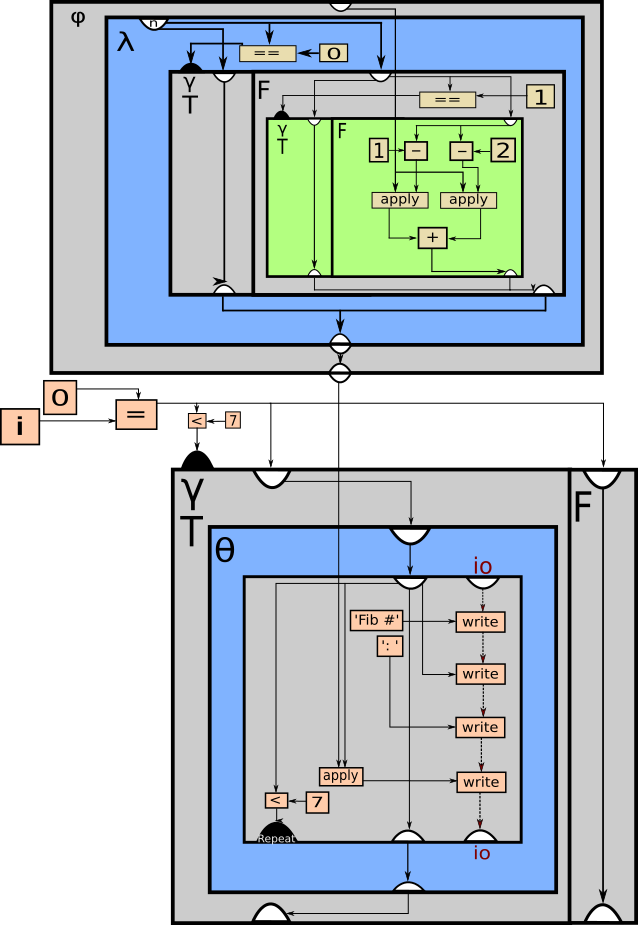
\includegraphics[width=\textwidth]{figures/for-loop-printf-rec_fib-example}
	\caption{A program consisting of a $\theta$-node looping 7 iterations,
calculating and printing the 7 first Fibonacci numbers. The \applyNode ~contained
in the $\theta$-node links to the same recursive Fibonacci function as in
Figure~\ref{fig:rec_fib_phi}.}
	\label{fig:factorial_for_loop_ex}
\end{figure}

\clearpage
\item \textbf{$\lambda$-nodes: Functions}

\textit{$\lambda$-nodes} represent functions. Their input are all dependencies
its subgraph depend upon\footnote{Of which any parameters the function the
$\lambda$-node represents needs is a subset.}. A $\lambda$-nodes' outputs need
to match the arity of the outputs the function it represents have, unless it is
a stateful function, in which case the $\lambda$-node has external outputs for
each side-effecting dependency.

However, $\lambda$-nodes themselves are never linked with anything but the
\applyNode s representing the call sites of the function the $\lambda$-node
represent. It is the \applyNode s which receive the input dependence edges and
give out the output dependence edges in an RVSDG. As previously mentioned, the
arity and order of inputs and outputs for the subgraph(s) inside the linked
$\lambda$-node must match the order and arity of the inputs and outputs of the
linked \applyNode .

\item \textbf{$\phi$-nodes: Recursive environments}

\textit{$\phi$-nodes}' subgraphs must contain at least one recursive
$\lambda$-node. As such, $\phi$-nodes have no external inputs, but they have
external outputs which represent links to each $\lambda$-node contained within.
The internal ``outputs'' of a $\phi$-region are links representing the
$\lambda$-nodes contained within, thus upholding the DAG properties of an RVSDG containing $\lambda$-nodes representing recursive functions.

All \applyNode s causing recursion inside a $\phi$-node get their first input
link from the ``internal input'' of the $\phi$-node which corresponds to the
$\lambda$-node the \applyNode represents a call site for. Hence, the
$\lambda$-nodes within do not extend any edges for their ``outer outputs'' from
their RVSDG subgraphs, such as non-recursive $\lambda$-nodes do. Instead, they
have one single output, which is linked to the internal ``inputs'' of the
$\phi$-node, which in turn are gated through to each its own external ``output''
in the $\phi$-node.

In this way, \applyNode s representing calls to the recursive functions
contained in the $\phi$-node, which are located elsewhere in the RVSDG, can get
their link to the $\lambda$-node representing function the \applyNode s
represent a call site of. A recursive fibonacci function represented as an RVSDG
illustrates the usage of a $\phi$-node in Figure~\ref{fig:rec_fib_phi}).

\end{itemize}

\begin{lstlisting}[label={lst:rec_fib_phi}, style=customcpp,
caption={C/C++ code corresponding to the RVSDG subgraph in
Figure~\ref{fig:rec_fib_phi}, which represents a simple recursive fibonacci
function.}]
int rec_fib(unsigned int n){
	if (n < 2){
		return n;
	}
	return rec_fib(n-1) + rec_fib(n-2);
}
\end{lstlisting}
\vspace{-4\parskip} %http://tex.stackexchange.com/q/40863

\begin{figure}[h!]
	\centering
	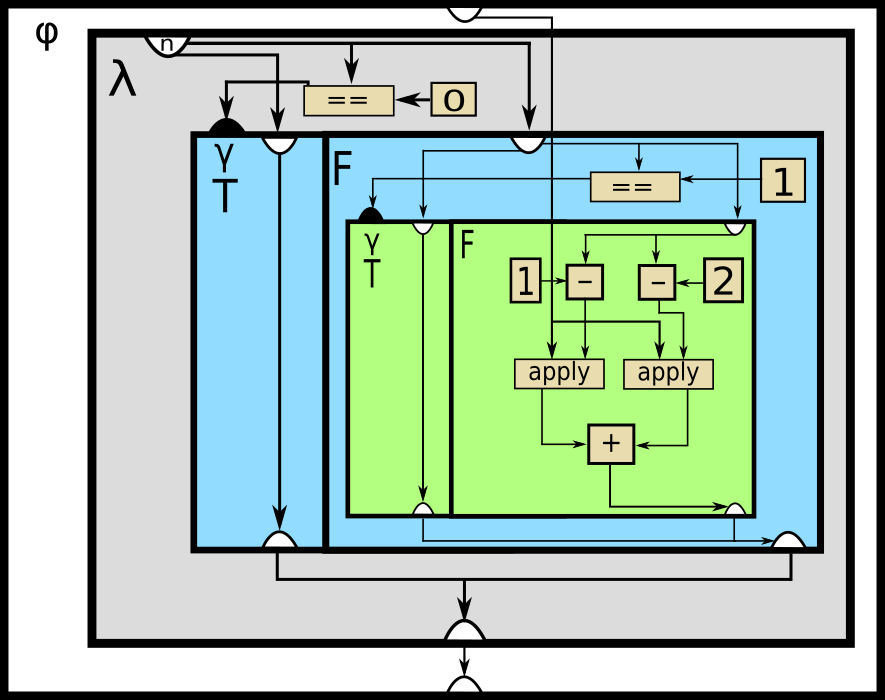
\includegraphics[width=\textwidth]{figures/recursive_fibonacci}
	\caption{A $\phi$-node containing a $\lambda$-node representing a recursive
version of a function producing the \lstinline!n! first numbers in the Fibonacci
series.}
	\label{fig:rec_fib_phi}
\end{figure}
